\label{literature_review}

\subsection{Thực trạng cháy nổ và an toàn lính cứu hỏa}

Quá trình đô thị hóa nhanh và sự xuống cấp của hạ tầng xây dựng đã làm gia tăng đáng kể nguy cơ cháy nổ tại các khu dân cư và khu công nghiệp \cite{Clarke2021firefighter, Fialho_Fire2024}. Nhiều công trình xây dựng không kiểm soát đã tạo ra những điểm yếu về an toàn trong khi hệ thống phòng cháy tại chỗ tại nhiều tòa nhà đã trở nên lỗi thời hoặc không đáp ứng yêu cầu hiện hành \cite{Rosengren_FIRE2014}. Những yếu tố này dẫn đến sự gia tăng về số lượng và mức độ nghiêm trọng của các vụ cháy nổ, đặt ra áp lực lớn lên lực lượng cứu hộ.

\begin{figure}[!htb]
    \centering
    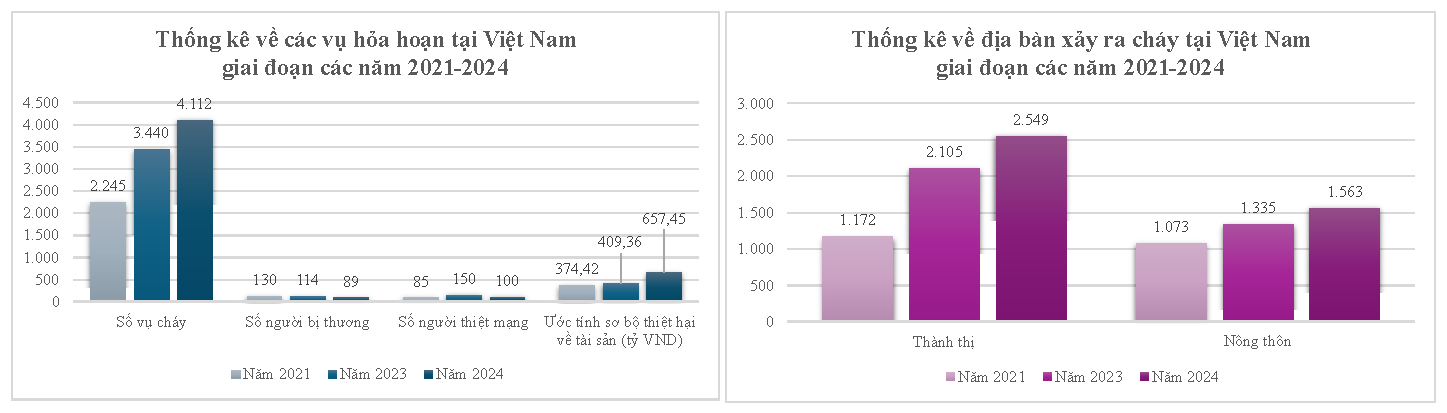
\includegraphics[width=0.85\linewidth]{Figure/tinh_hinh_chay_no.pdf}
    \caption{Thống kê tình hình cháy nổ qua các năm}
    \label{fig:tinh_hinh_chay}
\end{figure}

Lính cứu hỏa đóng vai trò then chốt trong các hoạt động ứng phó khẩn cấp và thường xuyên phải đối mặt với những nguy hiểm nghiêm trọng \cite{FirefighterImportant2022}. Các hiểm nguy phổ biến bao gồm nhiệt độ cực cao \cite{Firefighterhealthcare2024}, khí độc \cite{Firefighter_toxis}, không gian hẹp và nguy cơ sập đổ công trình. Theo thống kê của Hiệp hội Bảo vệ Phòng cháy Quốc gia Hoa Kỳ (NFPA), năm 2023 có 63.175 lính cứu hỏa bị thương với 89 trường hợp tử vong trong khi thi hành nhiệm vụ. Hoạt động dập tắt đám cháy chiếm tỉ lệ thương vong cao nhất, lên tới khoảng 18.875 trường hợp. Điều đáng chú ý là 87\% tổng số thương vong xảy ra trong các vụ cháy trong nhà, nơi xác suất thương tật vĩnh viễn cao gấp mười lần so với cháy ngoài nhà.

\begin{figure}[!htb]
    \centering
    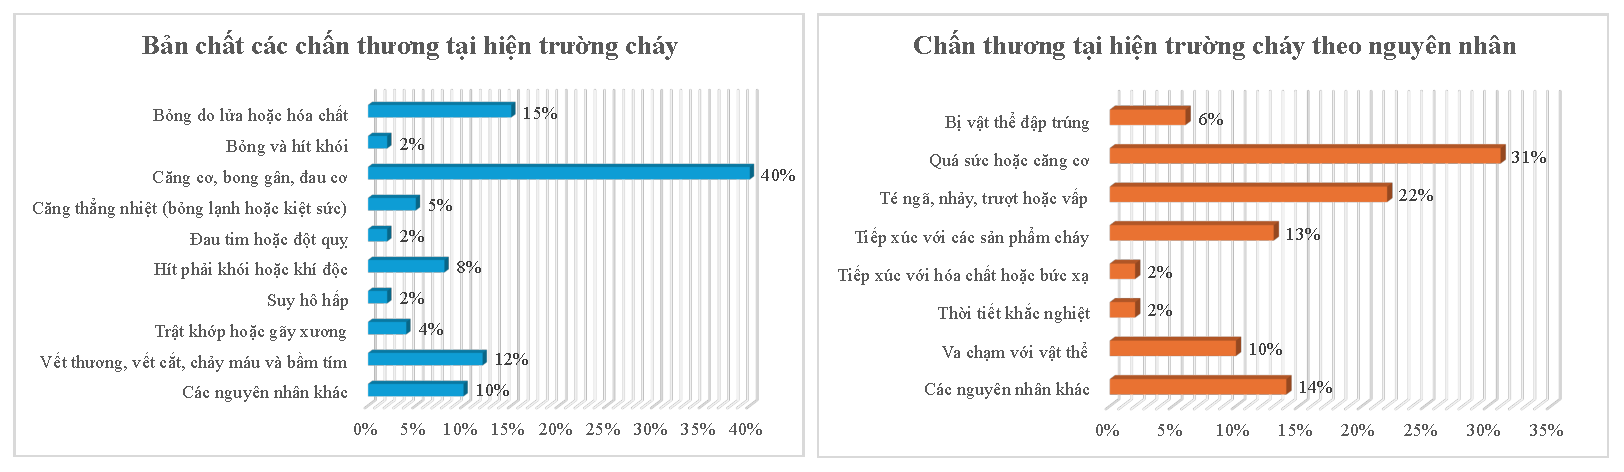
\includegraphics[width=0.85\linewidth]{Figure/nguyen_nhan_chan_thuong.pdf}
    \caption{Phân tích nguyên nhân chấn thương lính cứu hỏa}
    \label{fig:nguyen_nhan}
\end{figure}

Sự ứng dụng của khoa học công nghệ đã và đang nâng cao đáng kể mức độ an toàn của lính cứu hỏa \cite{FirefighterImportant2022, carmona2024firefighters}. Các hướng nghiên cứu chính hiện nay tập trung vào three lĩnh vực: (1) nâng cấp trang phục bảo hộ để giảm thiểu tác động của nhiệt và hóa chất \cite{FirefighterClothing2022}; (2) giám sát trạng thái tâm lý và sức khỏe trong điều kiện căng thẳng cao \cite{Firefighterhealthcare2024}; và (3) phát triển hệ thống giám sát hiện trường và liên lạc hỗ trợ ra quyết định \cite{Thanhfire2019, Firefighter_Falling_2023}.

\subsection{Tính cấp thiết của hệ thống giám sát hoạt động thời gian thực}

Việc giám sát liên tục hiệu suất hoạt động của lính cứu hỏa và duy trì liên lạc với trung tâm chỉ huy là yếu tố then chốt để phản ứng kịp thời và giảm thiểu rủi ro \cite{FirefighterImportant2022}. Tuy nhiên, các phương pháp liên lạc truyền thống như bộ đàm hai chiều chỉ cung cấp thông tin phân mảnh và thiếu khả năng theo dõi trạng thái theo thời gian thực của từng cá nhân \cite{Clifford2021}. Điều này gây cản trở đáng kể cho công tác phối hợp cứu hộ, đặc biệt khi không thể xác định vị trí hoặc trạng thái của một lính cứu hỏa do bất tỉnh hoặc bất động \cite{Zhang2024}.

Việc thiếu thông tin chính xác và liên tục về vị trí và trạng thái của từng lính cứu hỏa đặt ra những thách thức lớn cho công tác chỉ huy và phối hợp cứu hộ \cite{Firefighter_Falling_2023, Firefighterhealthcare2024}. Nhận dạng hoạt động lính cứu hỏa (FAR) kết hợp với thông tin vị trí là một hướng tiếp cận tiềm năng, cung cấp dữ liệu khách quan và liên tục, hỗ trợ ra quyết định kịp thời \cite{Accelerometerlocation2021}.

Khoảng trống nghiên cứu hiện tại thể hiện rõ ở ba điểm: (1) phần lớn nghiên cứu hiện có tập trung vào phát hiện ngã mà ít chú trọng đến nhận dạng toàn diện các hoạt động đặc thù của lính cứu hỏa như bò, trườn, đi khom; (2) thiếu tập dữ liệu công khai chuyên biệt cho lính cứu hỏa; (3) chưa có giải pháp tối ưu cho việc triển khai mô hình học máy trên vi điều khiển công suất thấp phù hợp với môi trường thi hành nhiệm vụ thực tế.

\subsection{Tổng quan nghiên cứu nhận dạng hoạt động con người}

\subsubsection{Phân loại phương pháp nhận dạng hoạt động}

Nhận dạng hoạt động con người được tiếp cận theo hai hướng chính: thị giác máy tính (computer vision) và tín hiệu cảm biến đeo (wearable sensor). Hướng thị giác máy tính gặp nhiều hạn chế trong môi trường chữa cháy thực tế do nhạy cảm với điều kiện ánh sáng và khói, yêu cầu xử lý dữ liệu phức tạp, đồng thời đặt ra lo ngại về quyền riêng tư \cite{HARvision2020}. Ngược lại, cảm biến đeo được đánh giá cao nhờ kích thước nhỏ gọn, chi phí thấp và khả năng phát hiện nhanh các thay đổi động học \cite{Accelerometer2021, DaoHieu2022, ViManhTuyen2024, HongNhung2023}.

\subsubsection{Học máy truyền thống trong nhận dạng hoạt động}

Học máy (ML) truyền thống được ứng dụng rộng rãi trong HAR nhờ tính đơn giản, phù hợp triển khai trên thiết bị đeo công suất thấp và khả năng cân bằng giữa chi phí, hiệu quả năng lượng và hiệu suất nhận dạng \cite{HongNhung2023, DaoHieu2022}. Thu và cộng sự \cite{Thu2022} đã triển khai cây quyết định (DT) để phân loại năm hoạt động cơ bản (nằm, ngồi, đứng, đi bộ, chạy bộ), đạt độ chính xác 99\% trên vi điều khiển ESP8266. Hong và cộng sự \cite{HongNhung2023} phát triển hệ thống tích hợp gia tốc kế, vi điều khiển công suất thấp và RF, đạt độ chính xác 99,2\% khi nhận dạng bốn trạng thái hoạt động cơ bản.

Lu và cộng sự \cite{Lu2020} đề xuất phương pháp HAR sử dụng một cảm biến gia tốc kế duy nhất, kết hợp đặc trưng toàn cục và cục bộ, đạt 93\% độ chính xác với các thuật toán GBDT, RF, KNN và SVM. Bên cạnh các đặc trưng miền thời gian, Preece và cộng sự \cite{preece2008_leutheuser2013_Lu2020} đã so sánh 14 loại đặc trưng từ tín hiệu gia tốc kế trên các miền thời gian, tần số và wavelet, xác nhận rằng đặc trưng miền tần số từ cảm biến đặt tại mắt cá chân cho phép phân loại tám hoạt động với độ chính xác tối đa 94\%.

\subsubsection{Học sâu trong nhận dạng hoạt động}

Học sâu (DL) thể hiện ưu thế vượt trội trong HAR nhờ khả năng tự động học đặc trưng từ tín hiệu cảm biến và mô hình hóa các mẫu hoạt động phức tạp \cite{DL2021_HAR_wearable}. Xu và cộng sự \cite{HAR_DCT_deeplearning2023} đề xuất cơ chế chú ý kênh dựa trên biến đổi cosine rời rạc (DCT) trong miền tần số, cải thiện hiệu suất mô hình ResNet lên 79,51\% trên UniMiB-SHAR. Qin và cộng sự \cite{HAR_CNN_2024} phát triển chiến lược học cộng tác với mô hình CLS-CNN-ResNest, đạt 99,12\% trên WISDM và hỗ trợ suy luận trực tiếp trên thiết bị thông qua cơ chế chia sẻ trọng số giữa các mạng con.

Tuy nhiên, học sâu thường đòi hỏi tài nguyên tính toán lớn, khiến chúng kém phù hợp với các thiết bị nhúng có tài nguyên hạn chế. Đối với các ứng dụng HAR thời gian thực, đặc biệt trên nền tảng vi điều khiển công suất thấp, ML truyền thống vẫn là lựa chọn thực tế hơn nhờ tính đơn giản, chi phí thấp và khả năng triển khai hiệu quả.

\begin{table}[!htb]
    \centering
    \caption{Tổng quan các nghiên cứu HAR sử dụng thiết bị đeo}
    \label{tab:har_overview}
    \footnotesize
    \renewcommand{\arraystretch}{1.2}
    \resizebox{\linewidth}{!}{
    \begin{tabular}{
        >{\centering\arraybackslash}m{0.08\linewidth}
        >{\RaggedRight\arraybackslash}m{0.52\linewidth}
        >{\RaggedRight\arraybackslash}m{0.12\linewidth}
        >{\RaggedRight\arraybackslash}m{0.22\linewidth}
    }
        \hline\hline
        \rowcolor{gray!20}\textbf{Năm} & \textbf{Tập dữ liệu} & \textbf{Đối tượng} & \textbf{Phương pháp} \\
        \hline\hline
        2024 & Accelerometer; UniMiB (50~Hz), WISDM (20~Hz), UCI (50~Hz); túi trước & Người, HĐ & CLS-CNN-ResNest \cite{HAR_CNN_2024}\\
        \hline
        2024 & Fusion sensors; 100~Hz; 18 TV; cánh tay, bắp tay, bắp chân; 8 HĐ & Lính CỐH, HĐ & Hybrid ML \cite{CHAI_FIRE2024}\\
        \hline
        2023 & Accelerometer; UniMiB (50~Hz), UR Fall (256~Hz), UCI (50~Hz) & Người, HĐ & CNN-DCT \cite{HAR_DCT_deeplearning2023}\\
        \hline
        2022 & Accelerometer, CO; 100~Hz; 8 TV; thắt lưng; 2 HĐ & Lính CỐH, ngã & Fall detection \cite{Dang2022}\\
        \hline
        2021 & 9-axis, 15~Hz; 10 TV; ngực, khuỷu, thắt lưng, đùi, mắt cá; 2 HĐ & Lính CỐH, ngã & LSTM \cite{Chai2021}\\
        \hline
        2020 & Accelerometer; 50~Hz; 21 TV; cổ tay; 6 HĐ & Người, HĐ & GBDT, RF, KNN, SVM \cite{Lu2020}\\
        \hline
        2019 & 9-axis, CO; barometer; 100~Hz; 6 TV; túi quần; 2 HĐ & Lính CỐH, ngã & Fall detection \cite{Thanhfire2019}\\
        \hline
        2016 & RF, doppler; 20~Hz; ngực, trán, cổ tay phải, mắt cá phải; 7 HĐ & Lính CỐH, HĐ & SVM \cite{Geng2016}\\
        \hline\hline
    \end{tabular}}
    \footnotesize \textit{Chú thích: TV = tình nguyện viên; HĐ = hoạt động; Lính CỐH = Lính cứu hỏa}
\end{table}

\subsection{Tổng quan nghiên cứu nhận dạng hoạt động lính cứu hỏa}

Hệ thống nhận dạng hoạt động lính cứu hỏa (FAR) phải xử lý các chuyển động động và cường độ cao trong môi trường nguy hiểm. Mục tiêu của các hệ thống này là nâng cao an toàn và hiệu quả hoạt động bằng cách giám sát thể chất, phát hiện bất thường và cung cấp thông tin thời gian thực trong tình huống khẩn cấp \cite{Firefighterhealthcare2024, Thanhfire2019}.

Geng và cộng sự \cite{Geng2016} giới thiệu phương pháp nhận dạng hoạt động lính cứu hỏa dựa trên tín hiệu tần số vô tuyến, sử dụng SVM với nhân Gaussian để phân biệt bảy hoạt động. Hệ thống đạt độ chính xác trung bình 88,7\%, trong đó các hoạt động tĩnh như đứng và nằm được nhận dạng chính xác hơn. Tuy nhiên, cửa sổ thời gian 10 giây hạn chế khả năng phản hồi nhanh với các hoạt động phức tạp và nhanh của lính cứu hỏa.

Pham và cộng sự \cite{Thanhfire2019} phát triển hệ thống hỗ trợ kết hợp thuật toán cảm biến hợp nhất để phát hiện ngã, giám sát tình trạng thể chất và đánh giá điều kiện môi trường. Thuật toán phát hiện ngã kết hợp dữ liệu gia tốc, tư thế và độ cao, đạt 100\% độ chính xác trên tập dữ liệu thực nghiệm riêng và 97,9\% trên tập dữ liệu công khai. Dang và cộng sự \cite{Dang2022} phát triển hệ thống hỗ trợ thời gian thực sử dụng gia tốc kế và cảm biến CO, đạt độ chính xác phát hiện ngã 93\% với độ nhạy 96,5\%. Chai và cộng sự \cite{Chai2021} phát triển hệ thống phát hiện ngã thông minh, tích hợp cảm biến vào trang phục bảo hộ tại năm vị trí cơ thể và sử dụng mạng LSTM ba lớp, đạt độ chính xác 94,1\%.

Nhìn chung, các nghiên cứu hiện tại chủ yếu tập trung vào phát hiện ngã mà chưa nhận dạng toàn diện các hoạt động đặc thù như bò (CR), trườn (SL), đi khom (WS). Hơn nữa, phần lớn nghiên cứu chưa giải quyết vấn đề nhận dạng chuyển tiếp giữa các hoạt động trong kịch bản thời gian thực, cũng như chưa tối ưu hóa cho triển khai trên vi điều khiển công suất thấp.

\subsection{TinyML và triển khai mô hình trên thiết bị biên}

TinyML là lĩnh vực nghiên cứu tập trung vào việc chạy suy luận học máy trực tiếp trên các thiết bị biên có tài nguyên hạn chế — thường có bộ nhớ Flash dưới 1~MB và RAM vài trăm KB \cite{SurveyTinyML2023}. Cách tiếp cận này mang lại lợi thế đáng kể về độ trễ thấp, tiết kiệm băng thông, tăng cường quyền riêng tư dữ liệu và khả năng hoạt động ngoại tuyến.

Saha và cộng sự \cite{MLforMicrocontroller2022} đã tổng quan các phương pháp học máy cho phần cứng cấp vi điều khiển, xác nhận rằng RF và các biến thể cây quyết định là nhóm thuật toán phù hợp nhất cho triển khai trên MCU điện năng thấp. Nghiên cứu của Vi và cộng sự \cite{ViManhTuyen2024} và Dao và cộng sự \cite{DaoHieu2022} đã chứng minh tính khả thi của việc triển khai RF trực tiếp trên vi điều khiển ESP32 và các MCU hiệu suất thấp tương tự, đạt hiệu suất nhận dạng cao với độ trễ chấp nhận được trong ứng dụng HAR thực tế.

Thư viện micromlgen cho phép chuyển đổi mô hình scikit-learn đã huấn luyện sang mã C/C++ tương thích với Arduino và ESP32, tạo điều kiện để tích hợp trực tiếp vào firmware thiết bị nhúng \cite{Tiny_machine_on_microcontroller}. Các nghiên cứu gần đây \cite{TinyMLOnEmbedded2025, RIOT_tinyML2025} xác nhận rằng các mô hình TinyML có thể hoạt động ổn định trong điều kiện tài nguyên hạn chế, với kích thước triển khai điển hình trong khoảng 0,5--1,0~MB flash.

\subsection{Mục tiêu, phạm vi và đóng góp của đề tài}

Dựa trên những khoảng trống nghiên cứu đã xác định, đề tài đặt ra mục tiêu xây dựng hệ thống RFAR --- hệ thống nhận dạng hoạt động lính cứu hỏa theo thời gian thực --- có khả năng phân loại chính xác mười một hoạt động đặc thù của lính cứu hỏa trong môi trường cứu hộ khẩn cấp, triển khai trên thiết bị đeo nhỏ gọn sử dụng vi điều khiển công suất thấp.

Đề tài hướng tới bốn đóng góp chính:

\begin{enumerate}[leftmargin=1.5cm, label=(\arabic*)]
    \item \textbf{Tập dữ liệu chuyên biệt:} Xây dựng tập dữ liệu mô phỏng các hoạt động lính cứu hỏa trong buổi diễn tập cứu nạn, bổ sung khoảng trống trong các tập dữ liệu công khai hiện có.
    \item \textbf{Quy trình xử lý tín hiệu mới:} Đề xuất pipeline kết hợp kỹ thuật cửa sổ trượt với phát hiện chỉ số bất thường (AIx) để cải thiện chất lượng thông tin hoạt động và xử lý hiệu quả các chuyển tiếp giữa hoạt động.
    \item \textbf{Hệ thống RFAR tối ưu:} Phát triển hệ thống sử dụng thiết bị đeo gia tốc kế tại thắt lưng để nhận dạng mười một hoạt động, triển khai mô hình RF tối ưu trên vi điều khiển công suất thấp với kích thước dưới 1~MB.
    \item \textbf{Thiết bị đeo thực tế:} Chế tạo thiết bị đeo có trọng lượng dưới 200~g, khả năng hoạt động liên tục 24~giờ, được xác nhận trong thực nghiệm thực tế với điểm F1$>$96\%.
\end{enumerate}

Về phạm vi của báo cáo tiến độ này, nghiên cứu đã hoàn thành các mục tiêu cốt lõi của giai đoạn hiện tại bao gồm xây dựng tập dữ liệu, phát triển và tối ưu hóa hệ thống, cùng thực nghiệm xác nhận. Các hướng mở rộng như tích hợp định vị trong nhà và mạng lưới giám sát tập trung đang được lên kế hoạch cho các giai đoạn tiếp theo.
